\chapter{Anexos}

\begin{landscape}
    \begin{figure}[H]
        \centering
        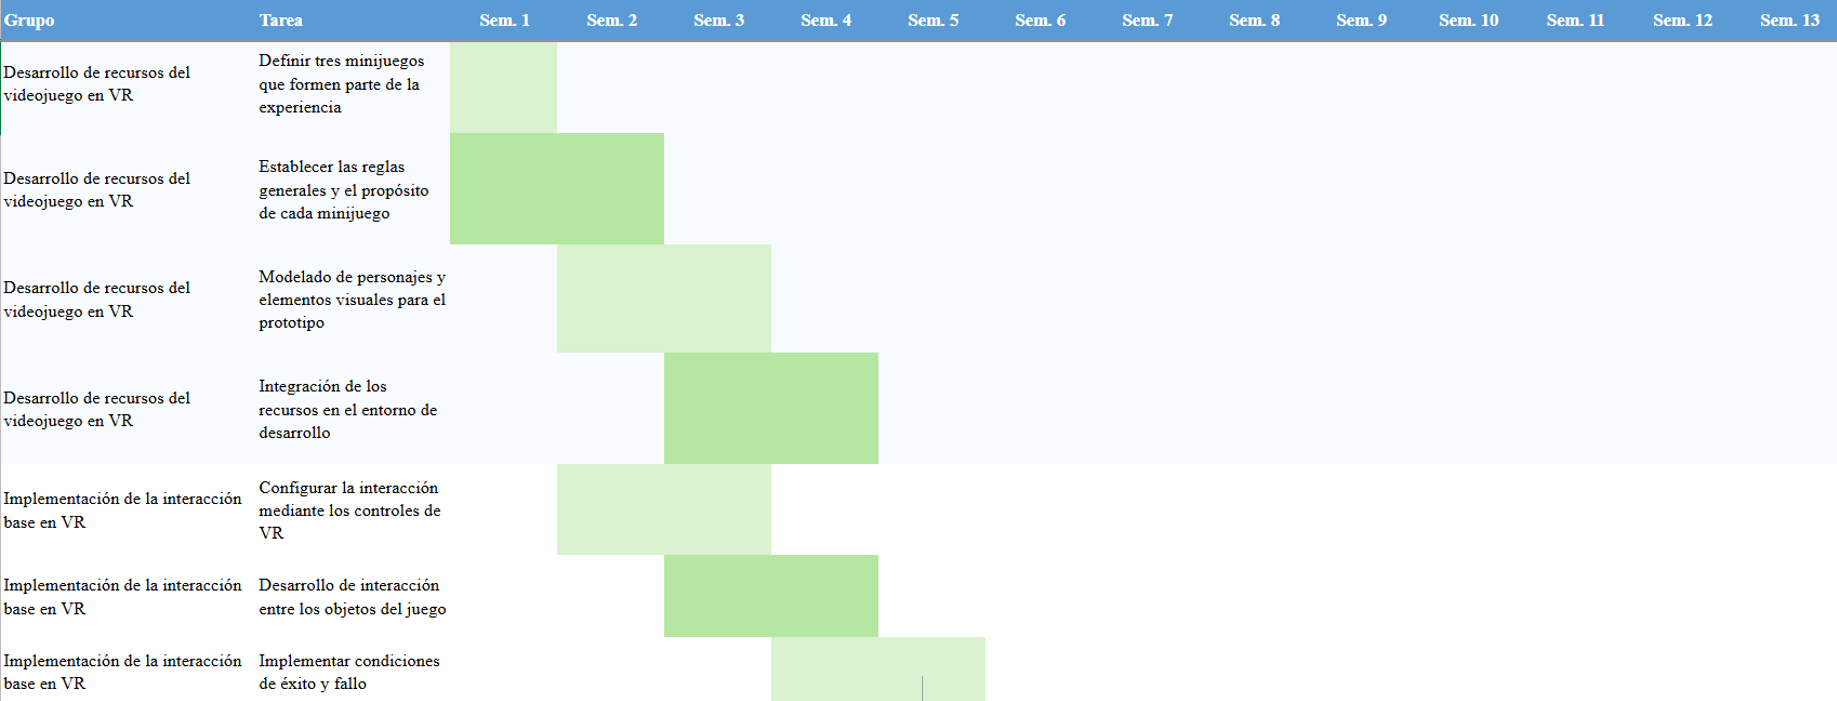
\includegraphics[
            width=\linewidth,
            height=0.80\textheight,
            keepaspectratio
        ]{imagenes/gantt1}
        \caption{Diagrama de Gantt para tareas parte 1}
        \label{fig:gantt1}
    \end{figure}
\end{landscape}

\begin{landscape}
    \begin{figure}[H]
        \centering
        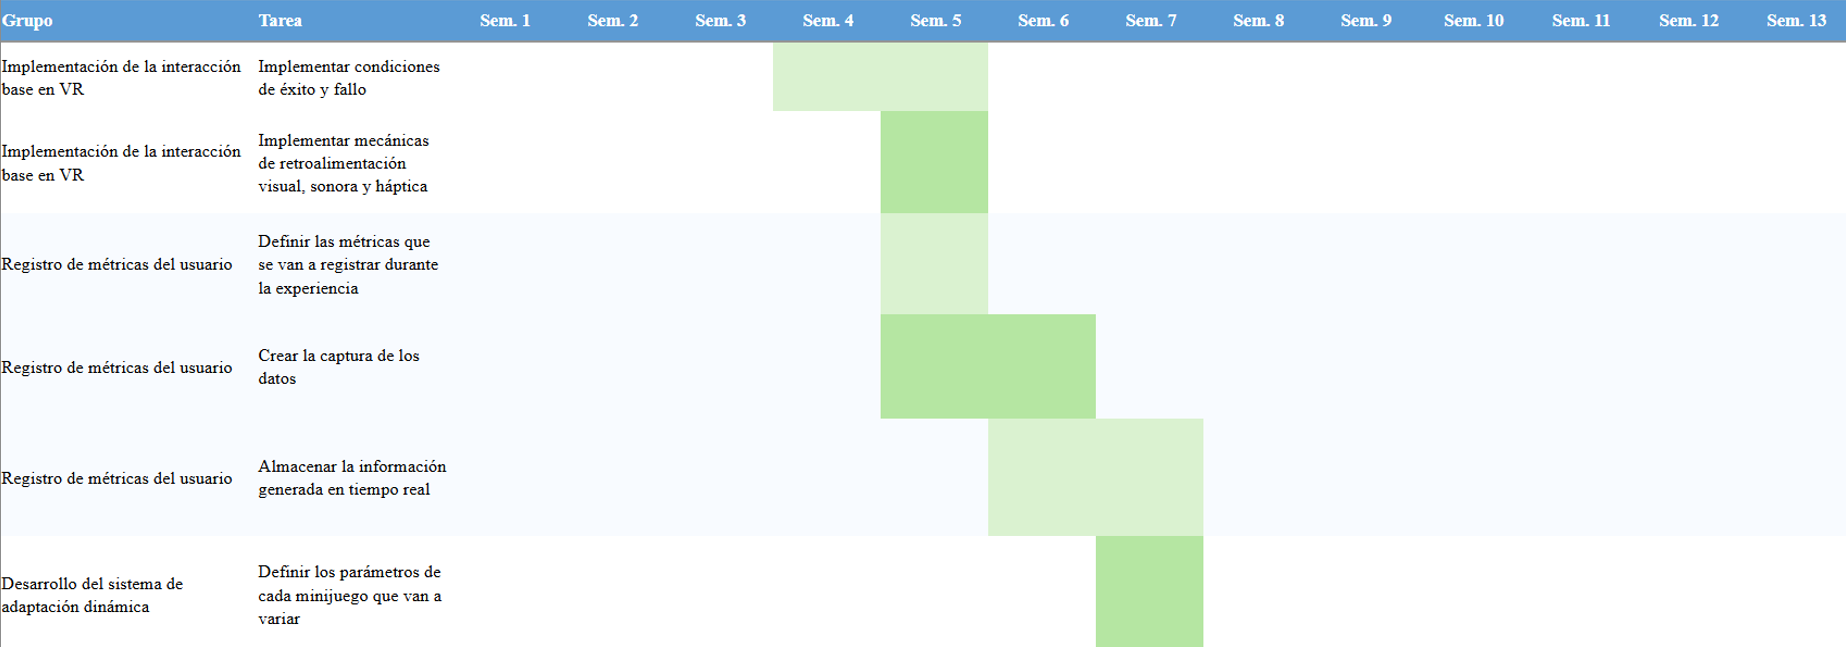
\includegraphics[
            width=\linewidth,
            height=0.80\textheight,
            keepaspectratio
        ]{imagenes/gantt2}
        \caption{Diagrama de Gantt para tareas parte 2}
        \label{fig:gantt2}
    \end{figure}
\end{landscape}

\begin{landscape}
    \begin{figure}[H]
        \centering
        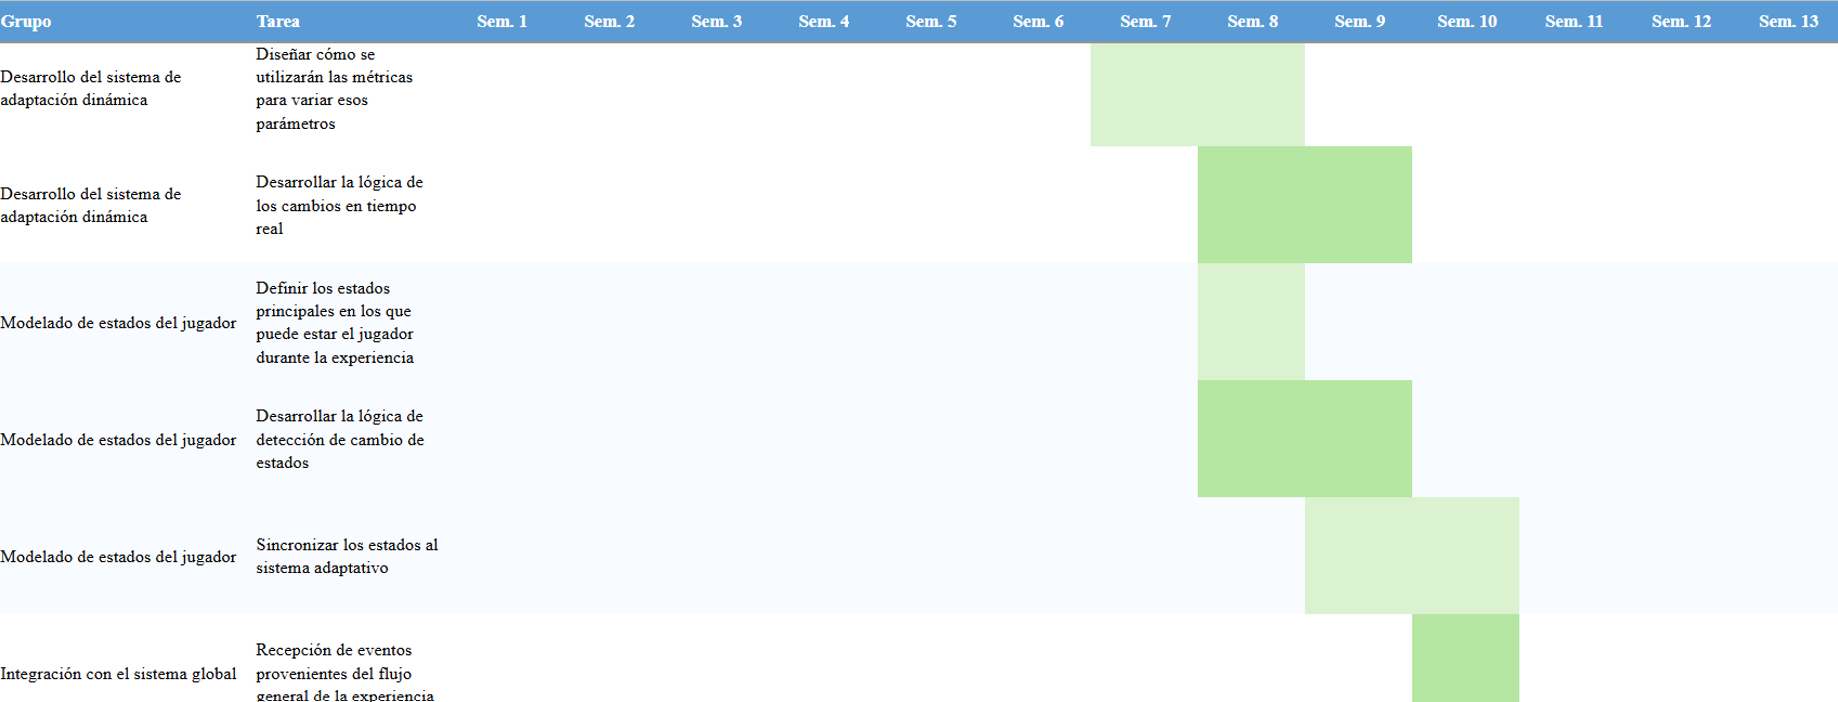
\includegraphics[
            width=\linewidth,
            height=0.80\textheight,
            keepaspectratio
        ]{imagenes/gantt3}
        \caption{Diagrama de Gantt para tareas parte 3}
        \label{fig:gantt3}
    \end{figure}
\end{landscape}

\begin{landscape}
    \begin{figure}[H]
        \centering
        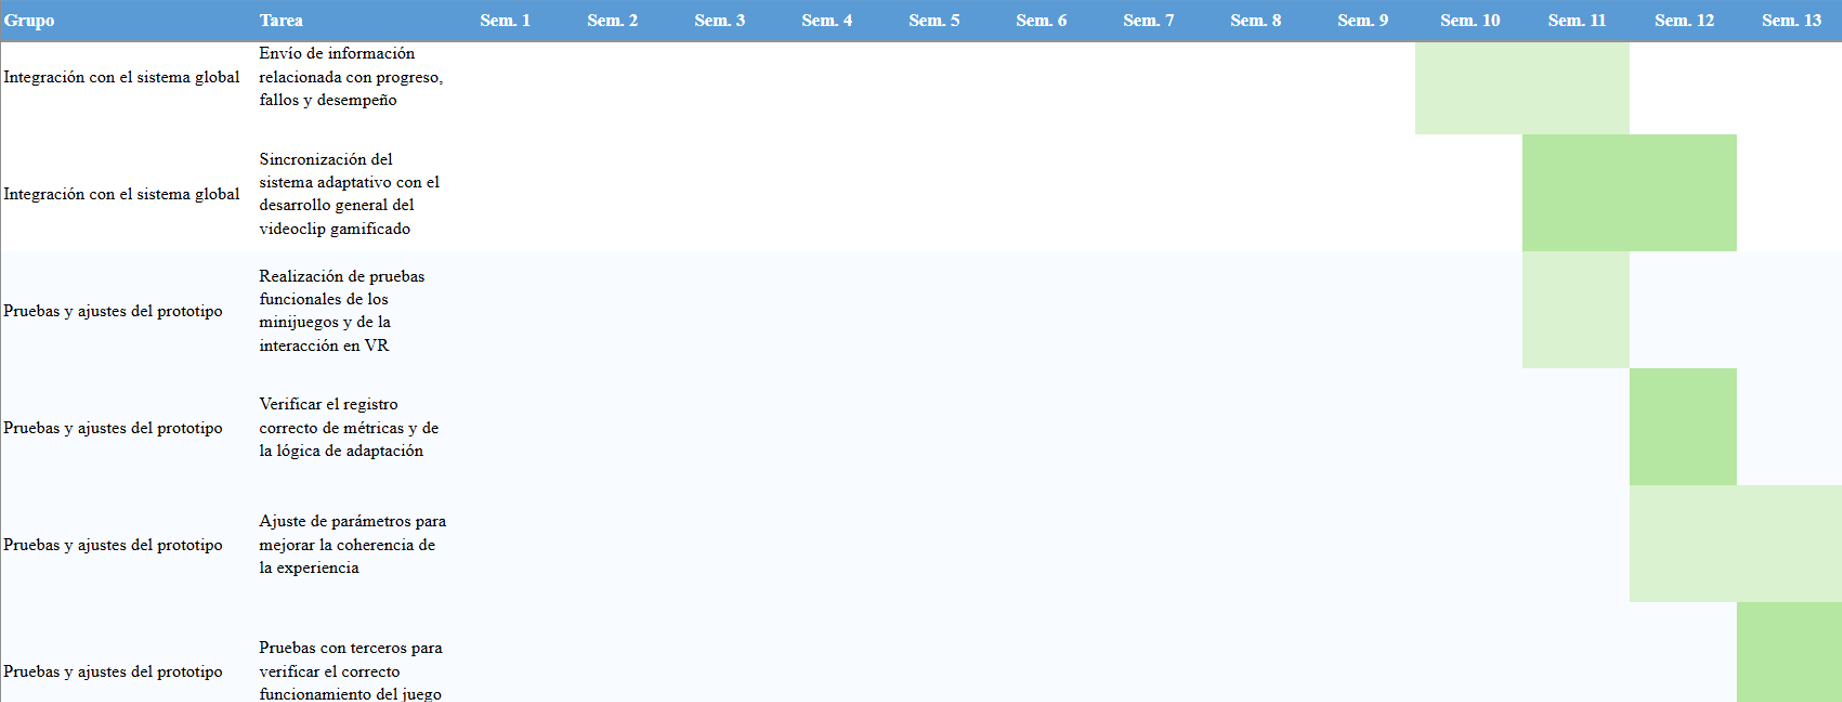
\includegraphics[
            width=\linewidth,
            height=0.80\textheight,
            keepaspectratio
        ]{imagenes/gantt4}
        \caption{Diagrama de Gantt para tareas parte 4}
        \label{fig:gantt4}
    \end{figure}
\end{landscape}